\section{Proposed Methodology}
\title{Proposed Methodology}
\begin{frame}{Proposed Methodology}

% 	\begin{columns}
	    
% 	    \column{.4\textwidth}
    	
%     	\column{.6\textwidth}
    
%     \end{columns}

    \begin{block}{General Concept}
        By the use of the concepts of Information Theory and Bayesian Networks it is intended to unite the method of Transfer Entropy and the K2 algorithm in order to generate a single methodology for the detection of causal relationships.
    \end{block}

    \begin{block}{Approach}
        To model  the system as a graph, in which the nodes will be the entities related to each other, by a causality
        relationship. This detection will be made in five stages.%: Generation of information flow graph, Application of Statistical Threshold, Removal of Cycles, Generation of Common and Virtual Ancestors, Modification and Computation of K2%
    \end{block}
\end{frame}

\begin{frame}{Proposed Methodology}
    \begin{figure}
        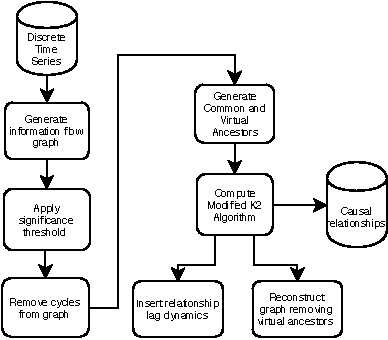
\includegraphics{figuras/methodology.pdf}
        \caption{Proposed Methodology}
    \end{figure}
\end{frame}
\subsection{Generation of graph of information flow}
\begin{frame}{Generation of graph of information flow}
    \begin{columns}
        \column{0.5\textwidth}
            \begin{itemize}
                \item{Given a system with N variables, it computes the Transfer Entropy pairwise for the set of variables.}

                \item{For each pair of variables, it computes the method \textit{h} times.}
                
                \item{It chooses the greatest entropy value from the \textit{h} computations.}
            \end{itemize}
        \column{0.5\textwidth}
            \begin{figure}
                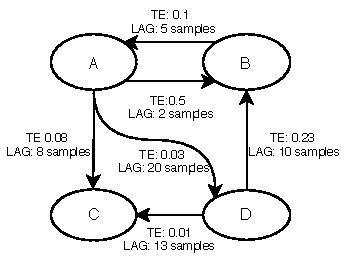
\includegraphics[width=\textwidth]{figuras/graphExample.pdf}
                \caption{Example of output from stage 1}
            \end{figure}          
    \end{columns}    

\end{frame}


\subsection{Application of Significance Threshold}
\begin{frame}{Application of Significance Threshold}
    \begin{itemize}
        \item { Because the Transfer Entropy is calculated pairwise, it can produce a dense graph. Since due to the noise contained in the time series,the chance of a zero entropy becomes low.
        }
        \item {In this stage is defined an empirical threshold for the relationships based on the distribution of the computed values.}
    \end{itemize}
\end{frame}

\begin{frame}{Application of Significance Threshold}
   \begin{figure}
                \centering
                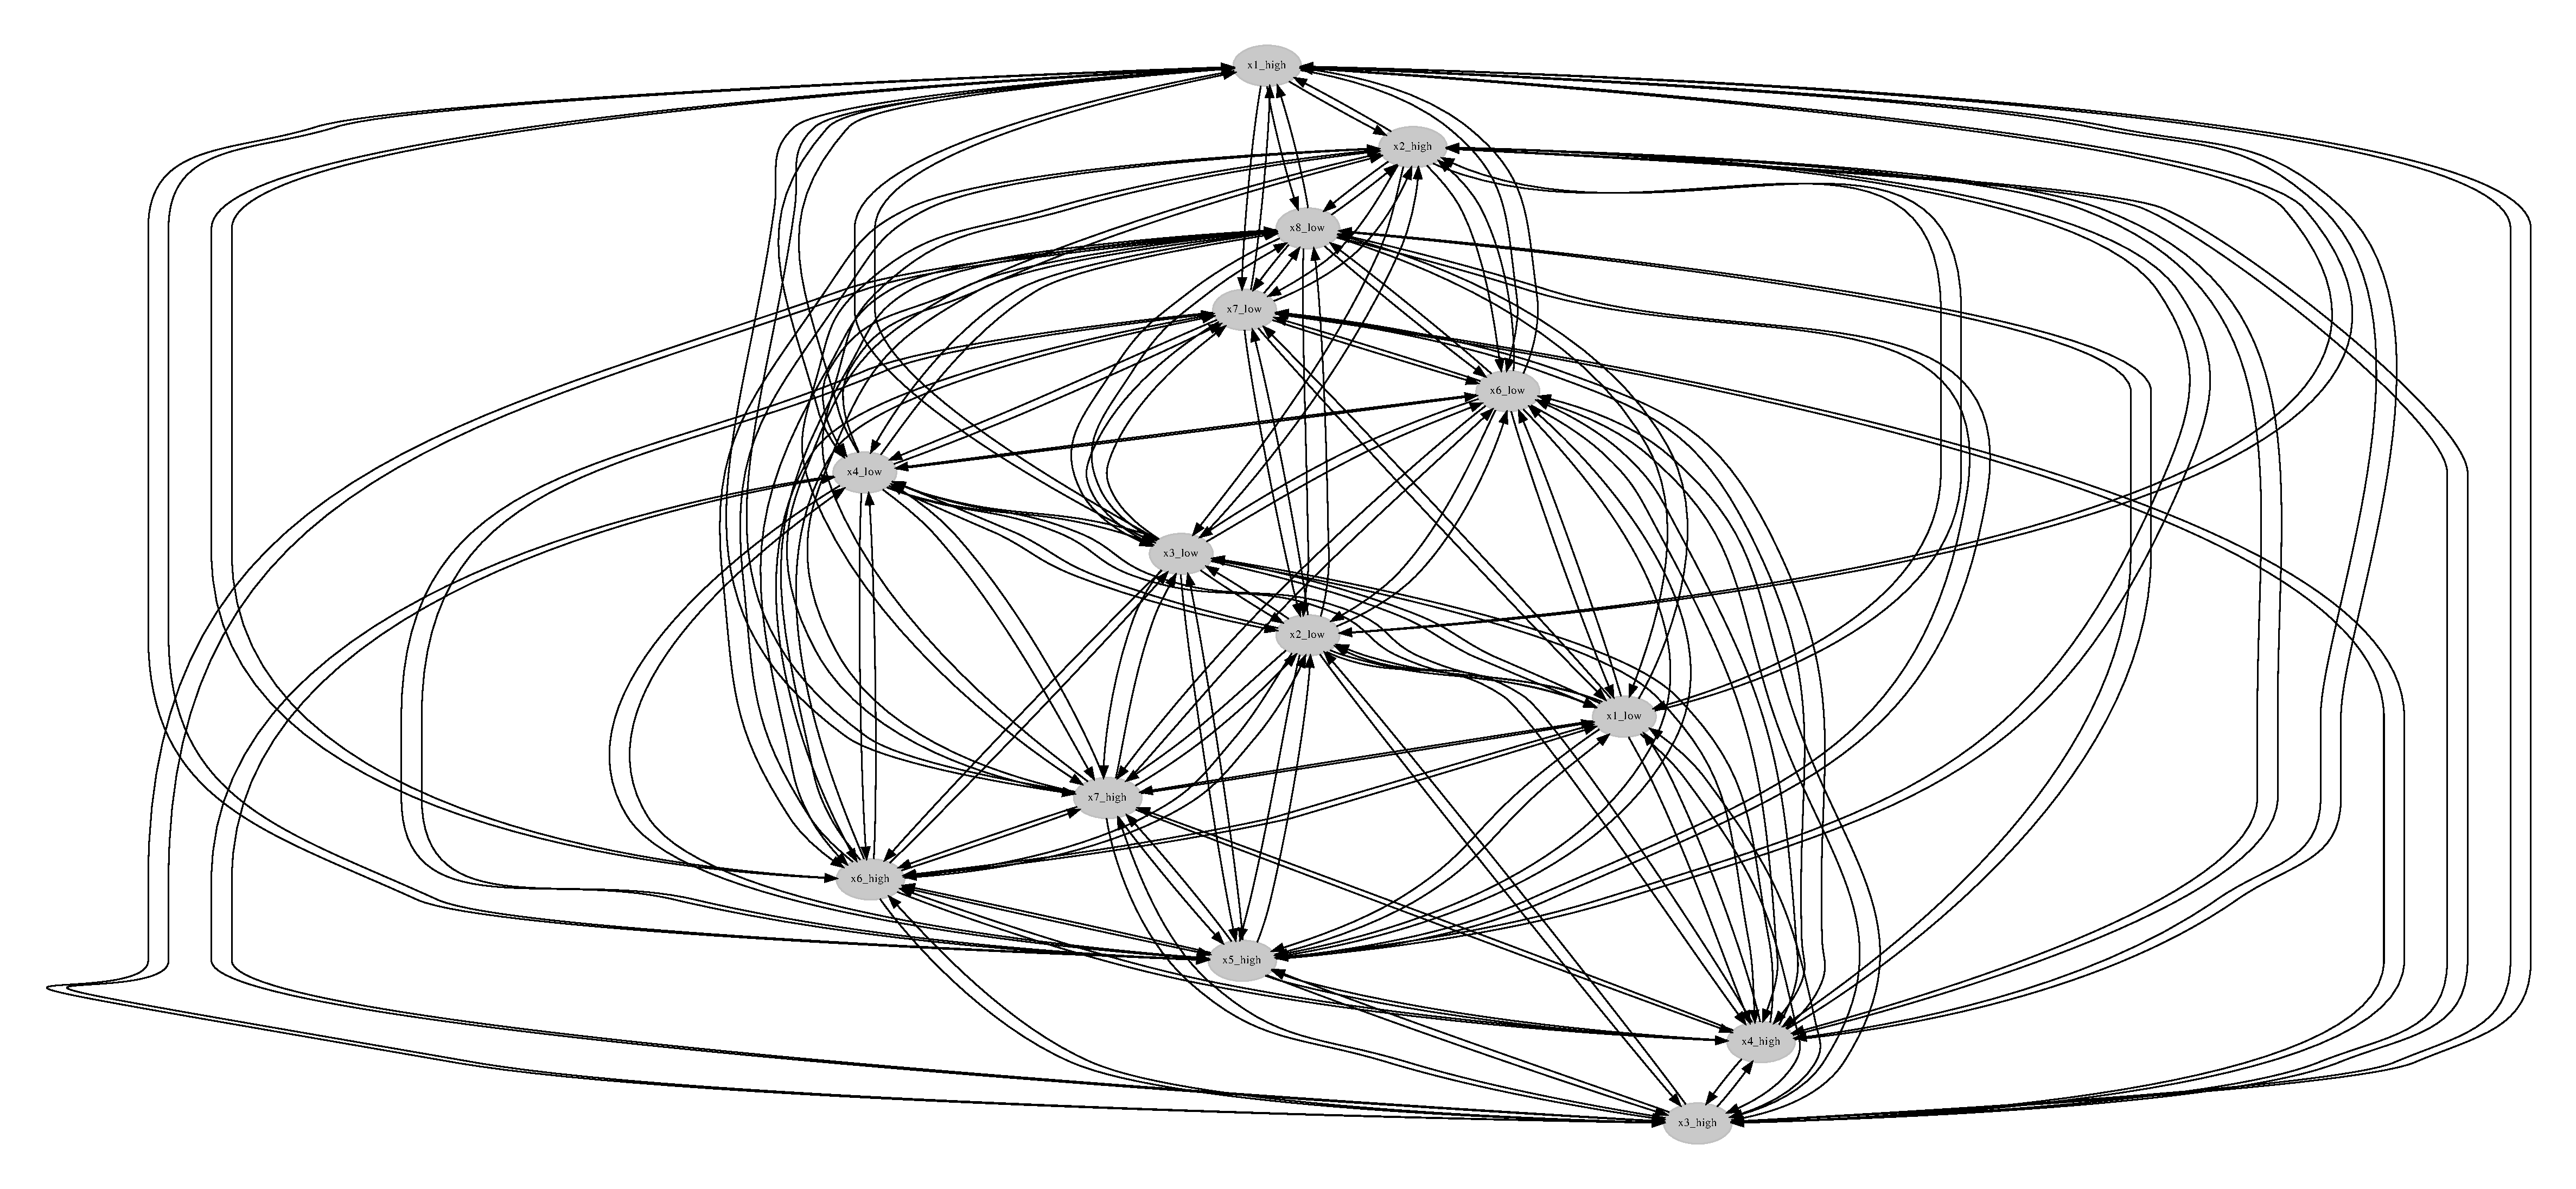
\includegraphics[width=\textwidth]{figuras/dot_graph.pdf}
                \caption{Transfer Entropy result without threshold}
                \label{fig:my_label}
            \end{figure}
\end{frame}

\begin{frame}{Application of Significance Threshold}
    \begin{figure}
        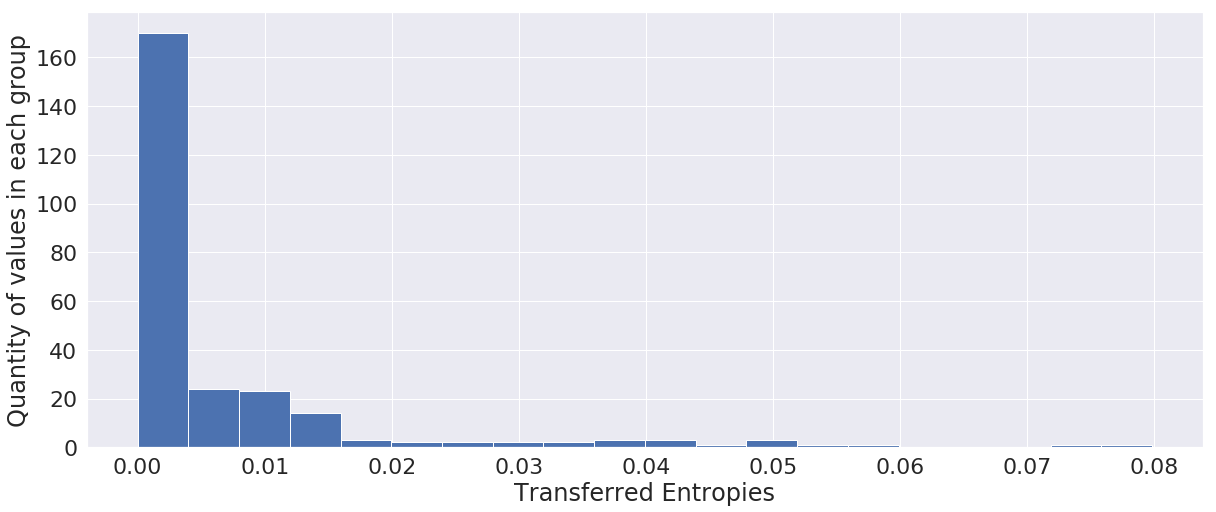
\includegraphics[width=\textwidth]{figuras/hist_ex.png}
    \end{figure}
\end{frame}

\begin{frame}{Application of Significance Threshold}
    \begin{figure}
        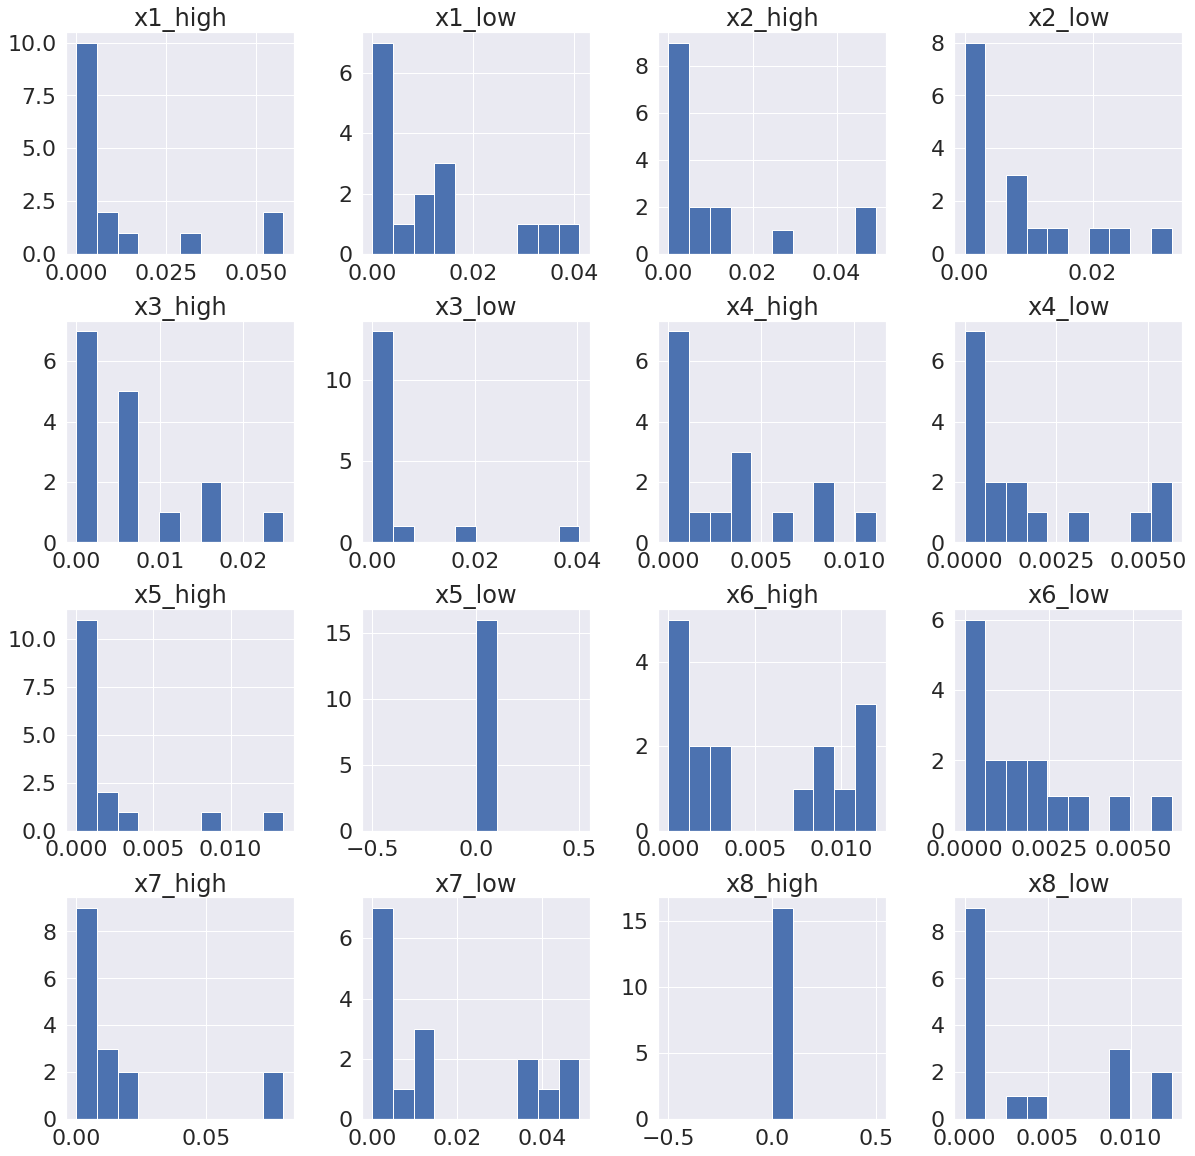
\includegraphics[width=0.8\textwidth, height=60mm]{figuras/mult_hist.png}
    \end{figure}

\end{frame}

% \begin{frame}{Application of Significance Threshold}
%     \begin{figure}
%         \includegraphics[width=0.8\textwidth, height=60mm]{figuras/exemplo_func.png}
%     \end{figure}

% \end{frame}

\begin{frame}{Application of Significance Threshold}
    \begin{figure}
        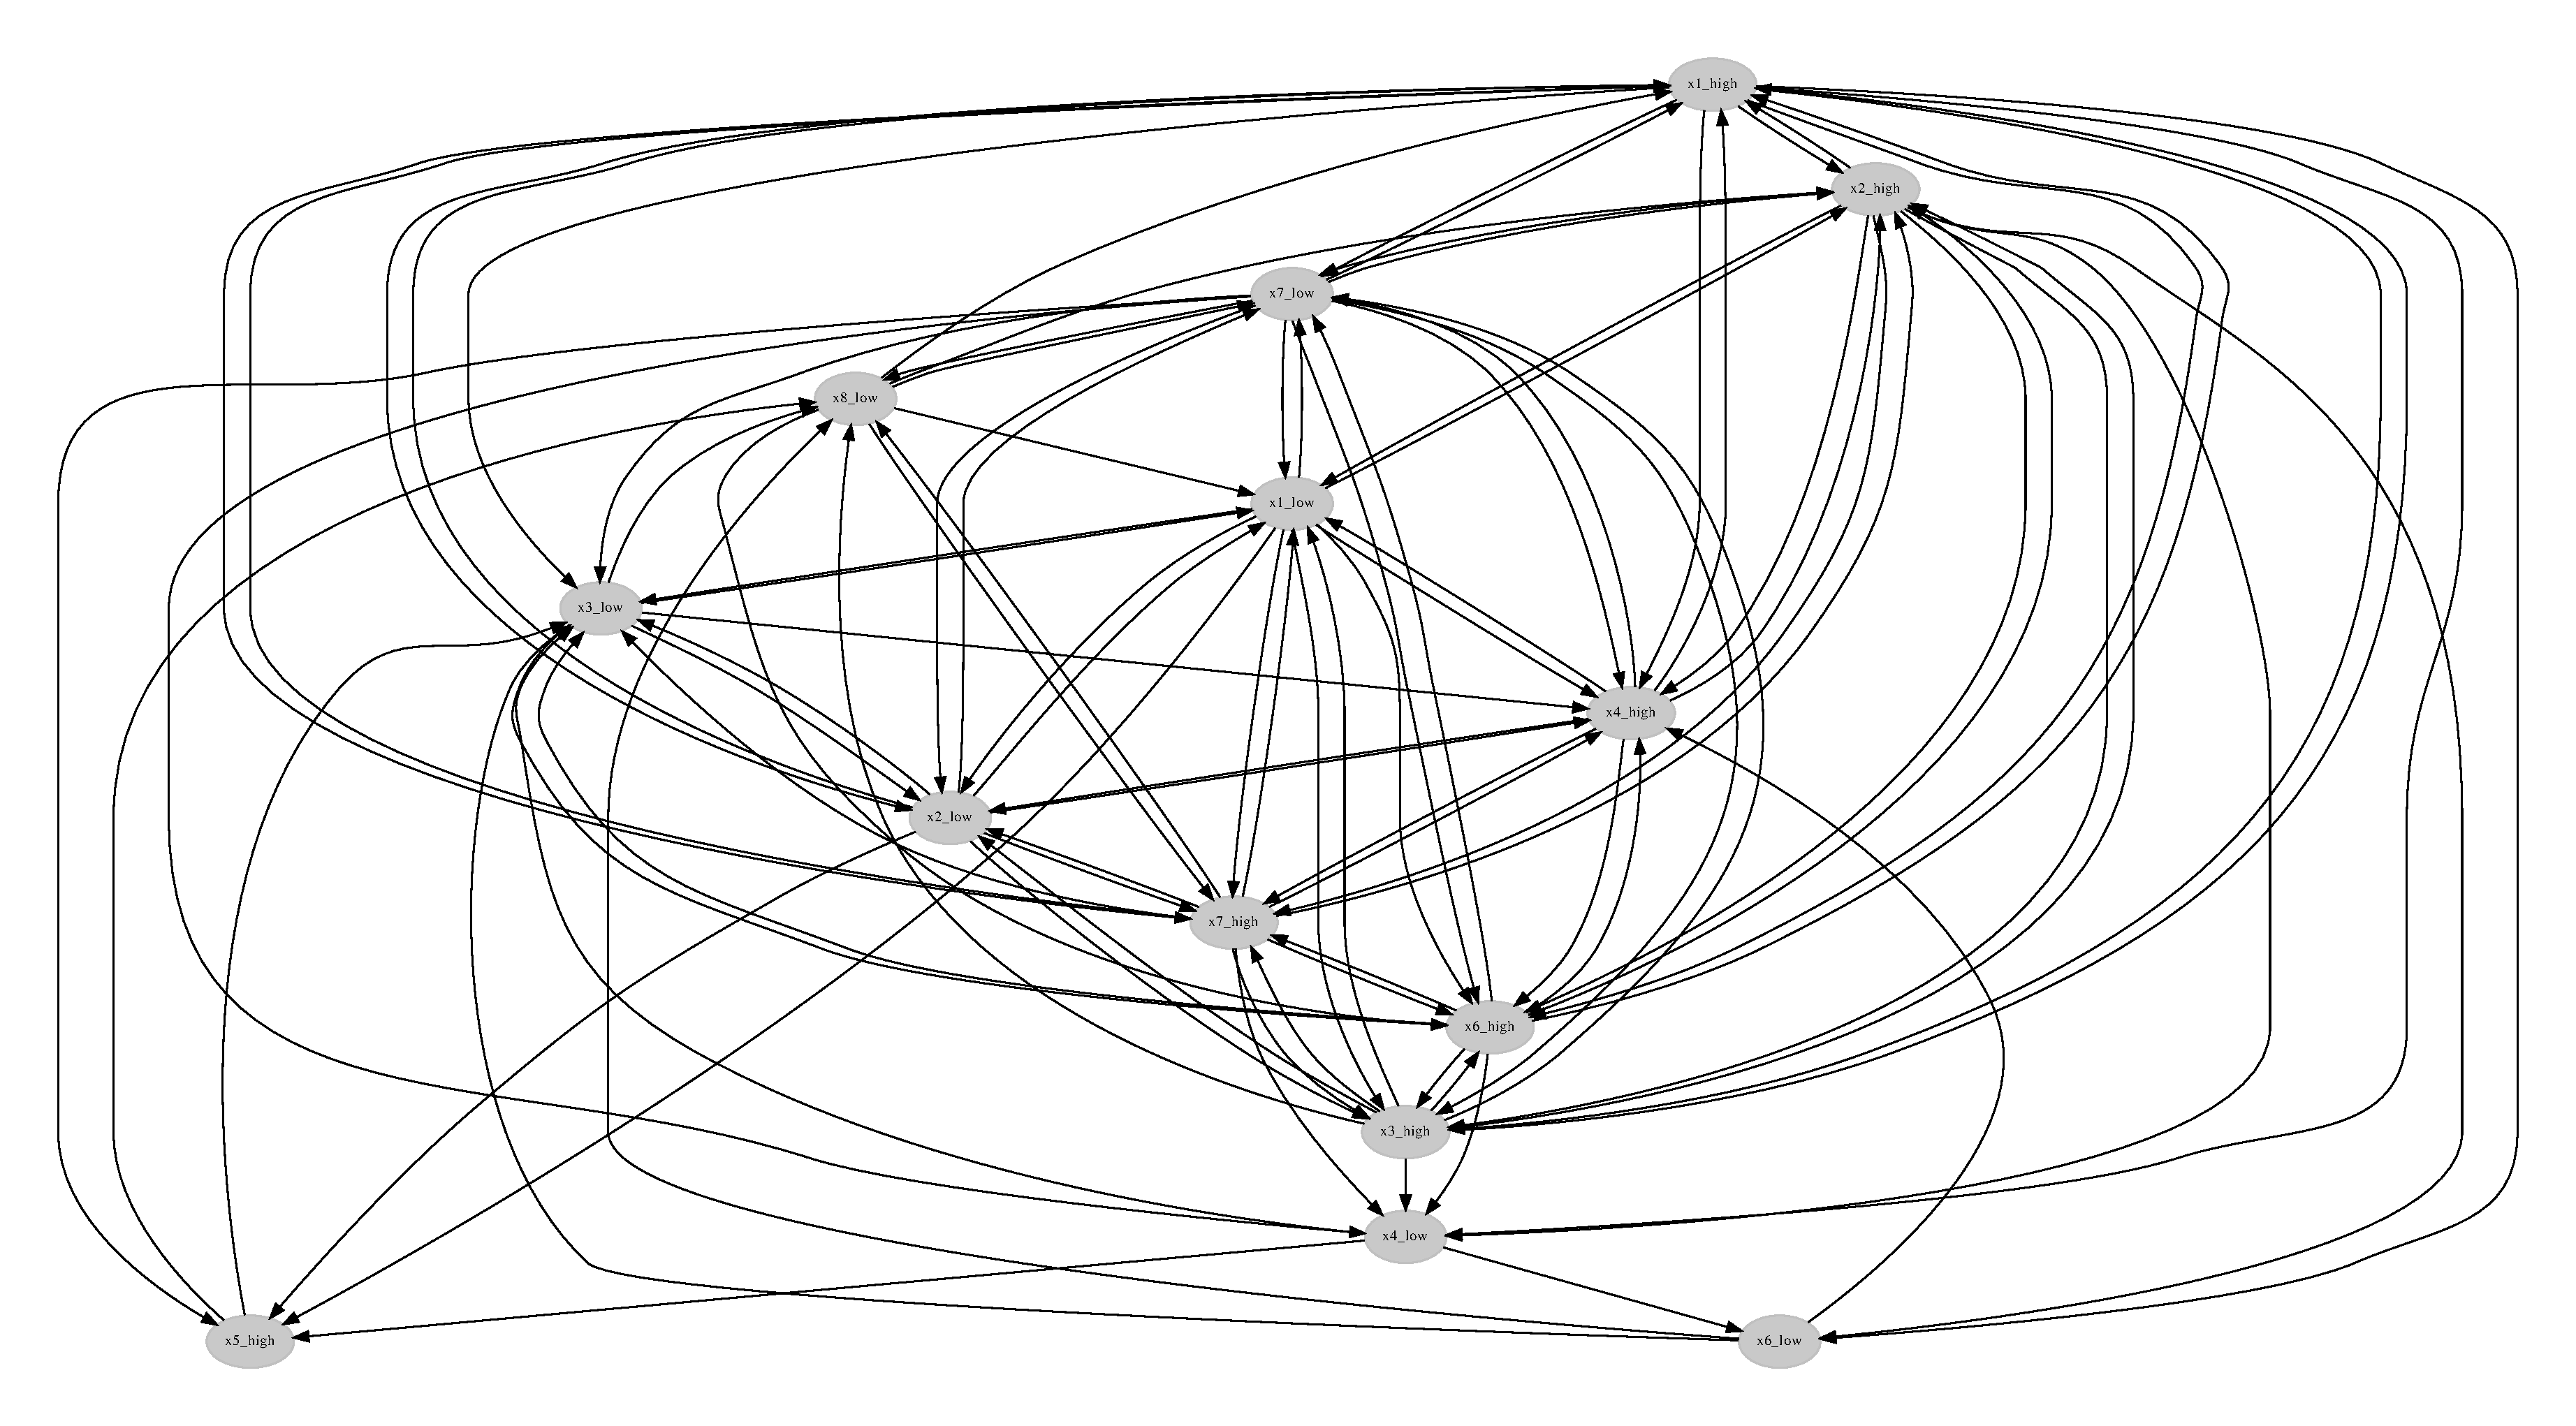
\includegraphics[width=0.8\textwidth, height=60mm]{figuras/vld_dot_graph.pdf}
        \caption{TE Graph after application of threshold.}
    \end{figure}
\end{frame}


\subsection{Removal of Cycles}
\begin{frame}{Removal of Cycles}
    \begin{itemize}
        \item { In order to prepare the graph to be used on K2, third stage does a removal of cycles.}
        \item Considering a selected relationship, it consists of recursive search on the graph, in which the nodes “above” the node-cause, are marked as its ancestors. Therefore, the ancestors of a node-cause cannot be related to it as an effect.
        \item {The removal is made based on the criterion of the higher information}
    \end{itemize}

\end{frame}


\begin{frame}{Removal of cycles}
    \begin{figure}
        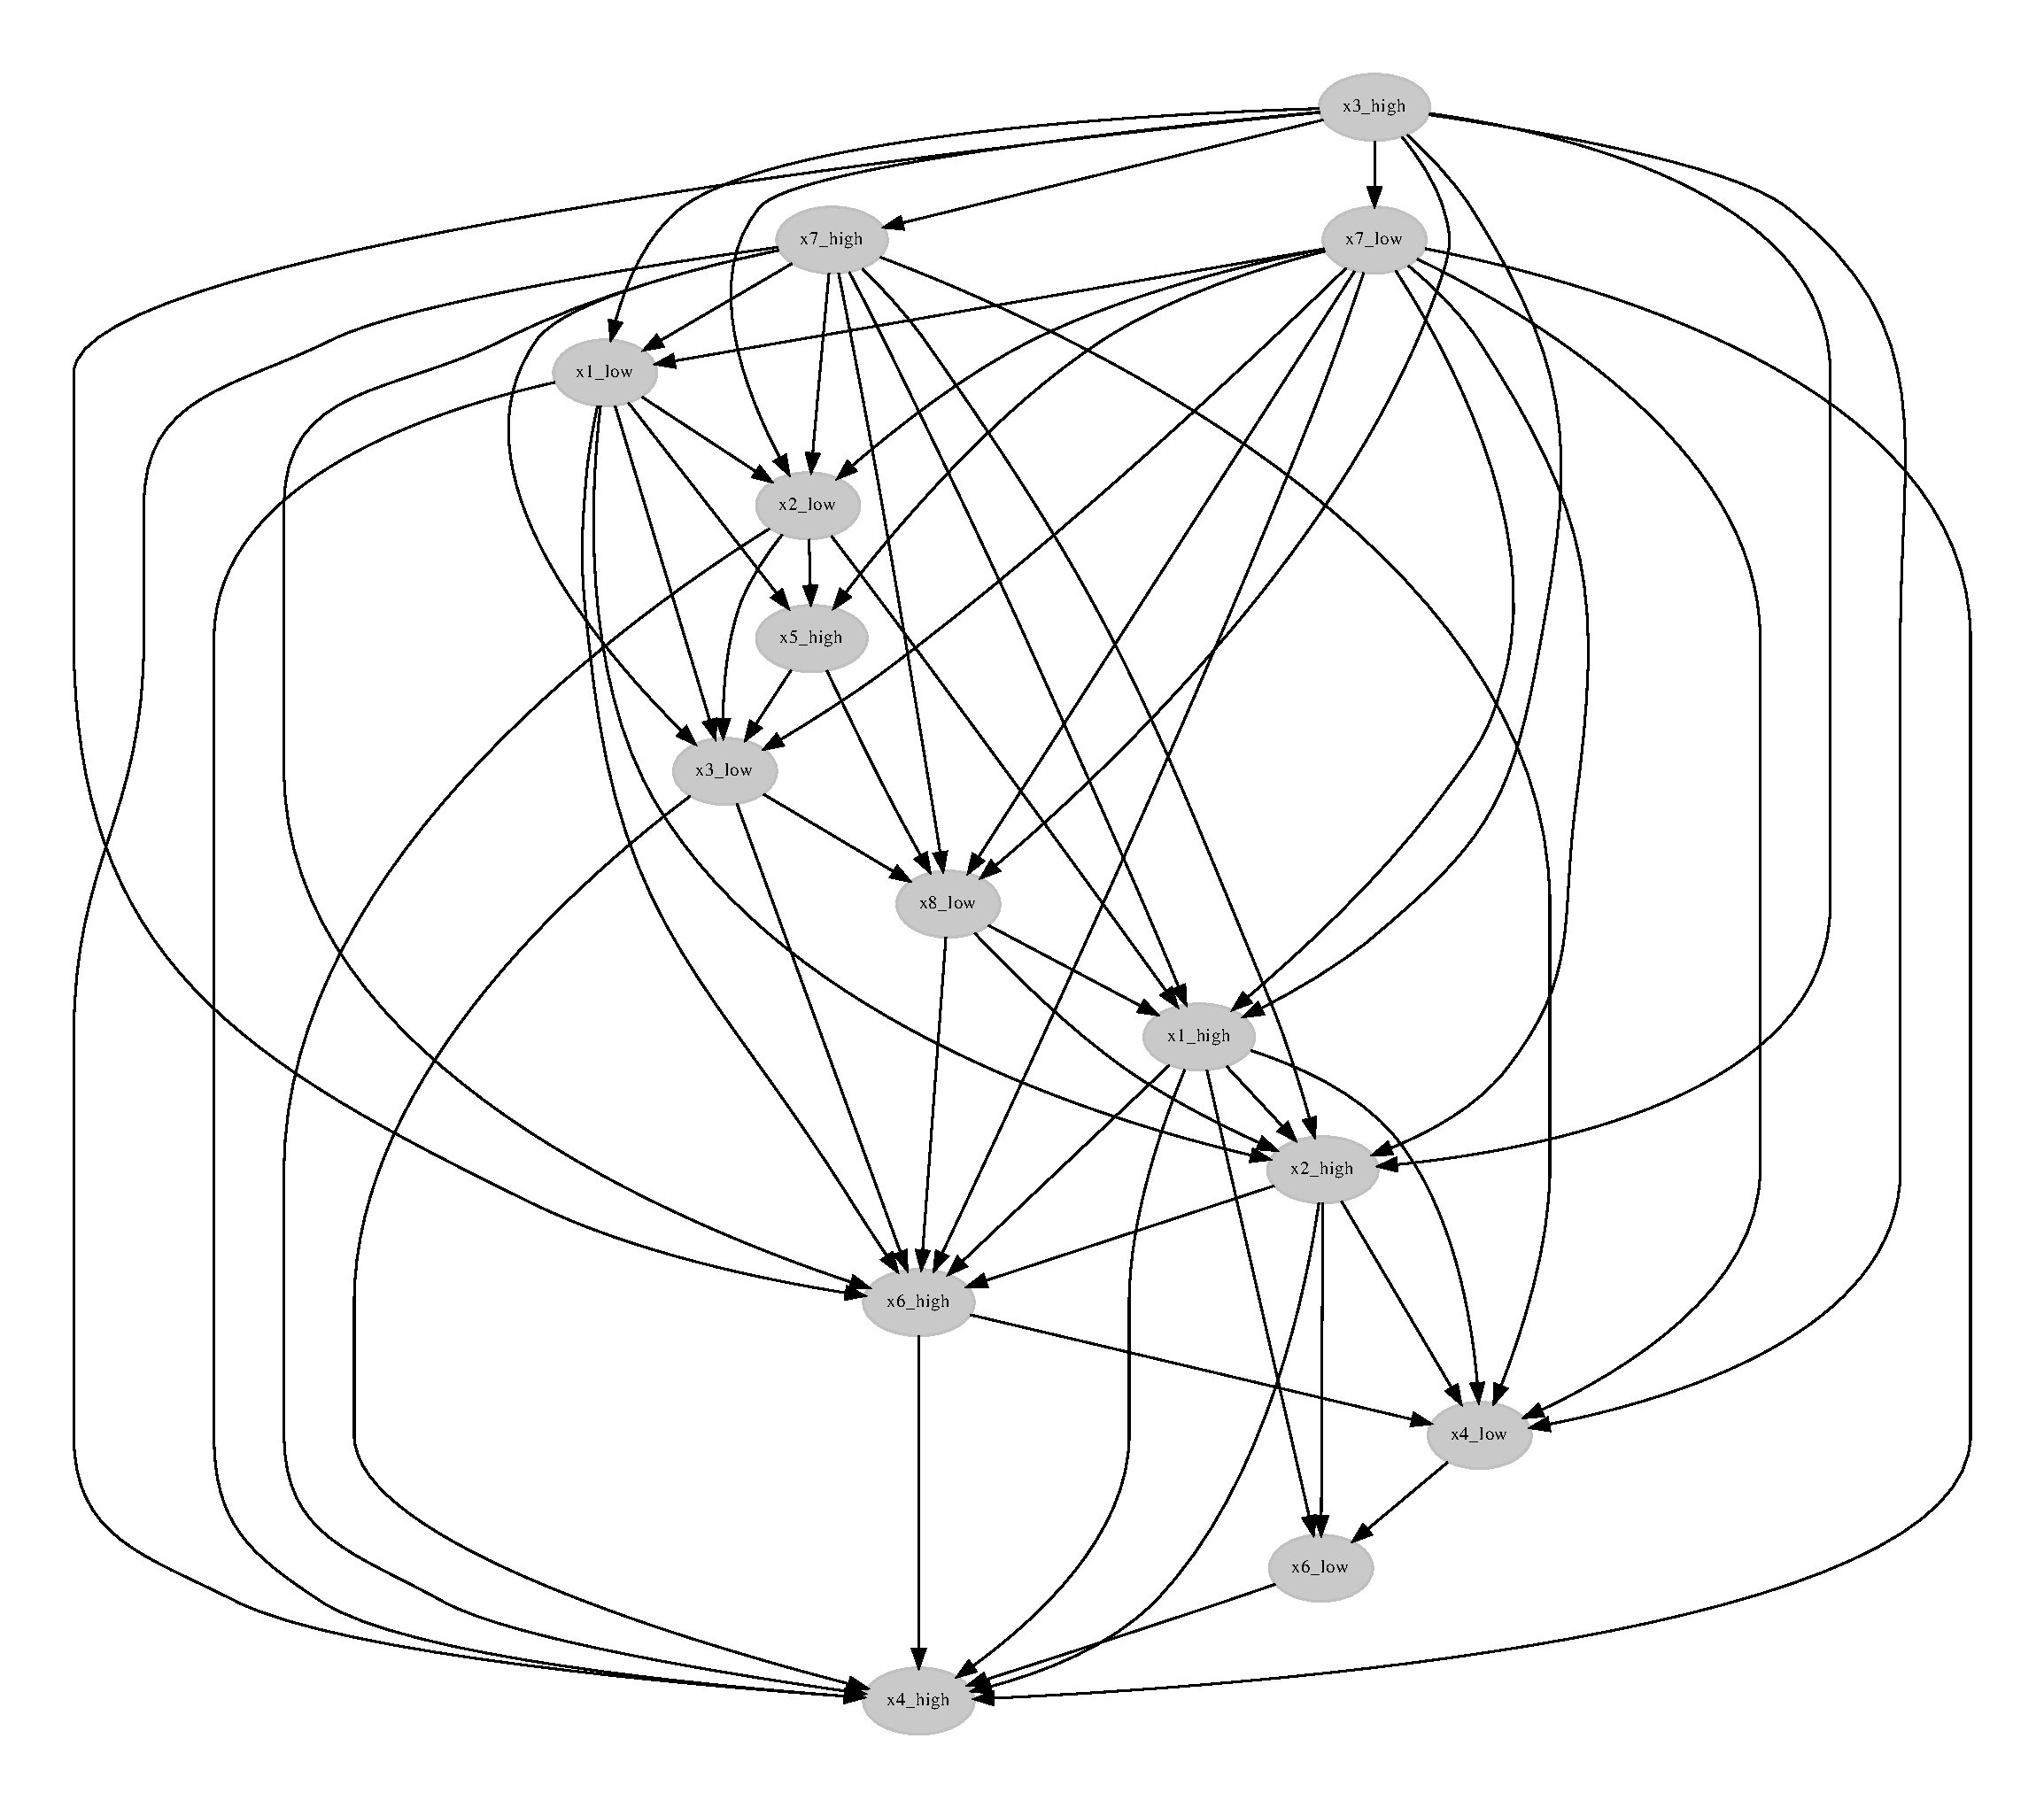
\includegraphics[width=0.8\textwidth, height=60mm]{figuras/grafo_ac_dot_graph.pdf}
        \caption{TE Graph without cycles.}
    \end{figure}
    
\end{frame}


\subsection{Generation of Common and Virtual Ancestors}
\begin{frame}{Generation of Common and Virtual Ancestors}

\textbf{What is a common and a virtual ancestor?}

\begin{columns}
    \column{0.5\textwidth}
        \begin{figure}
            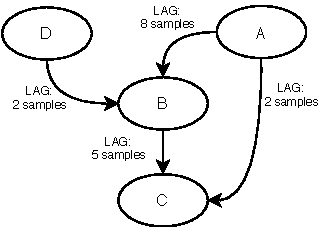
\includegraphics[width=\textwidth]{figuras/graphVirt.pdf}
            \caption{Ordinary Graph}
        \end{figure}
    \column{0.5\textwidth}
        \begin{figure}
            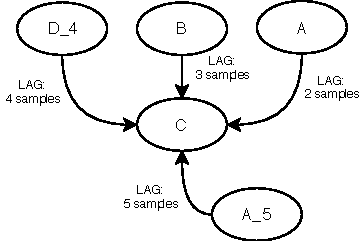
\includegraphics[width=\textwidth]{figuras/cVirt.pdf}
            \caption{Virtual and Common Ancestors}
        \end{figure}

\end{columns}
\end{frame}

\begin{frame}{Prior Structure to K2}
    \begin{columns}
        \column{0.5\textwidth}
                \begin{figure}
                    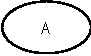
\includegraphics[height=2em]{figuras/aAnces.pdf}
                    \caption{A -  Ancestors}
                \end{figure}
                \begin{figure}
                    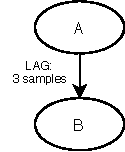
\includegraphics[height=5em]{figuras/bAnces.pdf}
                    \caption{B - Ancestors}
                \end{figure}
               
    \column{0.5\textwidth}
        \begin{figure}
            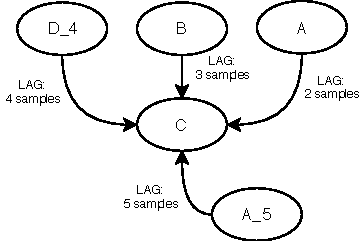
\includegraphics[width=\textwidth]{figuras/cVirt.pdf}
            \caption{C - Ancestors}
        \end{figure}
    \end{columns}
\end{frame}

\subsection{Modification and Computation of K2}
\begin{frame}{Modification and Computation of K2}

\begin{block}{Objectives}
\begin{itemize}
     \item To identify the most probable structure and therefore the flow of information.
    \item To reduce the number of arcs in the graph.
\end{itemize}
\end{block}


\begin{block}{Modifications}
\begin{itemize}
    \item The consideration of the common and virtual ancestors in the prior structure.
    \item The adequacy of the data sets, so that the relationships lags can be considered.
\end{itemize}
\end{block}
\end{frame}

\begin{frame}{Adequacy of the data set}
    \begin{columns}
        \column{\textwidth}
            \begin{figure}
                    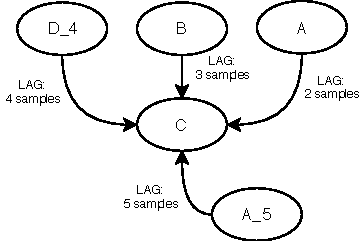
\includegraphics{figuras/cVirt.pdf}
                    \caption{C - Ancestors}
            \end{figure}
        
    \end{columns}
    
    
\end{frame}

\begin{frame}{Adequacy of the data set}
\begin{columns}\column{0.5\textwidth}%
    \centering
    \begin{figure}%
        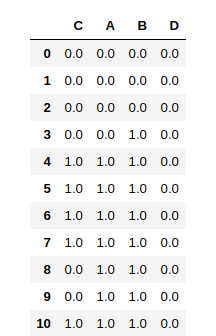
\includegraphics[height=.7\textheight]{figuras/cBefore.png}
        \caption{Before modification}
    \end{figure}
    \column{0.5\textwidth}
    \begin{figure}
        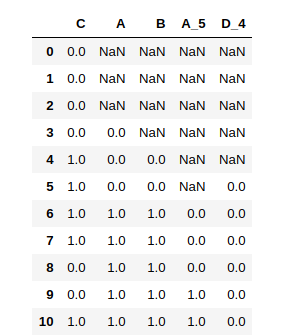
\includegraphics[height=.7\textheight]{figuras/cAfter.png}
        \caption{After modification}
    \end{figure}
\end{columns}
\end{frame}


\begin{frame}{Reconstruction of the Graph}
    \begin{columns}
        \column{0.5\textwidth} 
            \begin{itemize}
                \item Due to the addition of the virtual nodes the graph retrieved can contain relationships that does not correctly represent the indirect relationships among the nodes, as well as its respective lags.
            \end{itemize}
        \column{0.5\textwidth} 
            \begin{figure}
                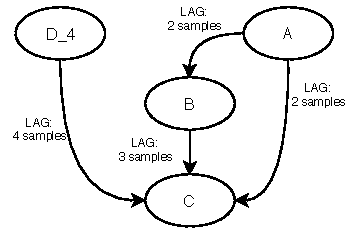
\includegraphics{figuras/recGraph.pdf}
                \caption{K2 Modified - Output}
                \label{fig:my_label}
            \end{figure}
    \end{columns}
    
\end{frame}